\documentclass{segabs}
\usepackage{xspace,color,amsmath,bm}
\usepackage{amssymb}
\usepackage{hyperref}

\begin{document}

\title{Comparison of magnetic vector inversion with sparse norm susceptibility inversion accounting for demagnetization}

%author{
%    John M. Weis$^1$, Lindsey J. Heagy$^1$ Douglas W. Oldenburg$^1$ \\
%    $^1$Geophysical Inversion Facility, University of British Columbia \\
%}
%\email{jweis@eoas.ubc.ca}

% \footer{Example}
%\lefthead{Weis, Heagy, Oldenburg}
%\righthead{Inversion methods to account for demagnetization}

\maketitle

\begin{abstract}
%\vspace{-0.6cm}

Self-demagnetization effects complicate the interpretation of magnetic data for highly susceptible targets by altering both the magnitude and direction of the resultant total magnetization. While magnetic vector inversion (MVI) can model self-demagnetization effects, the number of model parameters is tripled as compared to isotropic susceptibility inversion, increasing the non-uniqueness of the inverse problem. We show that if appropriate prior information is available, modeling demagnetization in terms of susceptibility can improve recovered models.  We apply sparse inversion with bound constraints to adequately simulate self-demagnetization effects, and compare results with compact MVI on a synthetic model.

\end{abstract}

%\vspace{-0.45cm}
\section{Introduction and motivation}
%\vspace{-0.25cm}

Magnetic geophysical surveys are diagnostic of the magnetization of the subsurface. If there is no remanent magnetization, the relationship between the resultant magnetization $\mathbf{M}$ and susceptibility $\chi$ is: \begin{equation}
    \mathbf{M} = \chi\mathbf{H}
    \label{eq:Mfull}
    % \vspace{-0.05cm}
\end{equation}
where $\mathbf{H}$ is composed of the primary geomagnetic field $\mathbf{H_0}$ and a secondary magnetic field $\mathbf{H_S}$. Standard susceptibility inversions assume that $\mathbf{H_S}$ plays a negligible role in induced magnetization as compared to the primary field. The relationship between the subsurface susceptibility and magnetization is then approximated as: \vspace{-0.1cm}
\begin{equation}
    \mathbf{M} = \chi\mathbf{H_0}
    \label{eq:Mlinear}
    \vspace{-0.05cm}
\end{equation}\citep{Li1996}. This assumes a uniform magnetization in the direction of the ambient geomagnetic field and is only applicable if the magnetic susceptibility $\mathbf{\chi}$ is low. Because a linear relationship is assumed between $\mathbf{M}$ and $\chi$, we refer to the associated forward modeling and inversion as linear in the remainder of this paper.

If the magnetic susceptibility is high, the secondary term $\chi \mathbf{H_S}$ is significant. For an isolated body, this term tends to reduce the magnetization in comparison to the linear approximation. This phenomenon is therefore often called self-demagnetization.  Even for a uniformly susceptible body, $\mathbf{H_s}$ varies depending on the shape of the body and how the body intersects the ambient geomagnetic field.  As a result, $\mathbf{H_s}$ does not in general run anti-parallel to $\mathbf{H_0}$, and self-demagnetization can have the effect of rotating the direction of magnetization away from the inducing field. Using standard susceptibility inversion when demagnetization effects are present will therefore not only underestimate the susceptibility of the subsurface but can also recover susceptible material in the wrong location.

Two forward modeling and inversion algorithms fully model the physics of demagnetization. The first is MVI \citep{Lelievre2009} which inverts for the total magnetization and makes no assumption on the cause of magnetization. Although MVI can model remanence, demagnetization, and anisotropy, the recovered model $\mathbf{M}$ is a vector field. Therefore, the discrete magnetization model contains 3 parameters per cell, adding non-uniqueness to the inverse problem.  The second algorithm inverts in terms of scalar susceptibility and is capable of modeling the demagnetization effect \citep{Lelievre2006}.  This accounts for a  nonlinear relationship between $\mathbf{M}$ and $\chi$, and we refer to the associated forward modeling and inversion as nonlinear in the remainder of this paper. We compare the two methods on a synthetic plate model inspired by the Osborne deposit in Queensland, Australia and demonstrate that for compact and highly susceptible bodies, nonlinear susceptibility inversion can outperform MVI if appropriate prior information is available.

%\vspace{-0.45cm}
\section{Forward Modeling}
%\vspace{-0.25cm}

We develop a finite-volume forward modeling and inversion code capable of modeling high-susceptibility and remanence or total resultant magnetization (MVI) using the open-source framework SimPEG \citep{Cockett2015}. We forward model data for a plate-like ironstone body inspired by the Osborne deposit, which has a uniform susceptibility of $\chi=6$ SI and no remanent magnetization (Figure \ref{fig:magnetization}). The plate dips at a $45^{\circ}$ angle and extends a total of 200 meters in the $y$ direction.  The ambient geomagnetic field has a strength of $52000$nT, a $-55^{\circ}$ inclination, and a $45^{\circ}$ declination from clockwise from the $+y$ direction.

\begin{figure}[htb]
    \vspace{-0.1cm}
    \begin{center}
    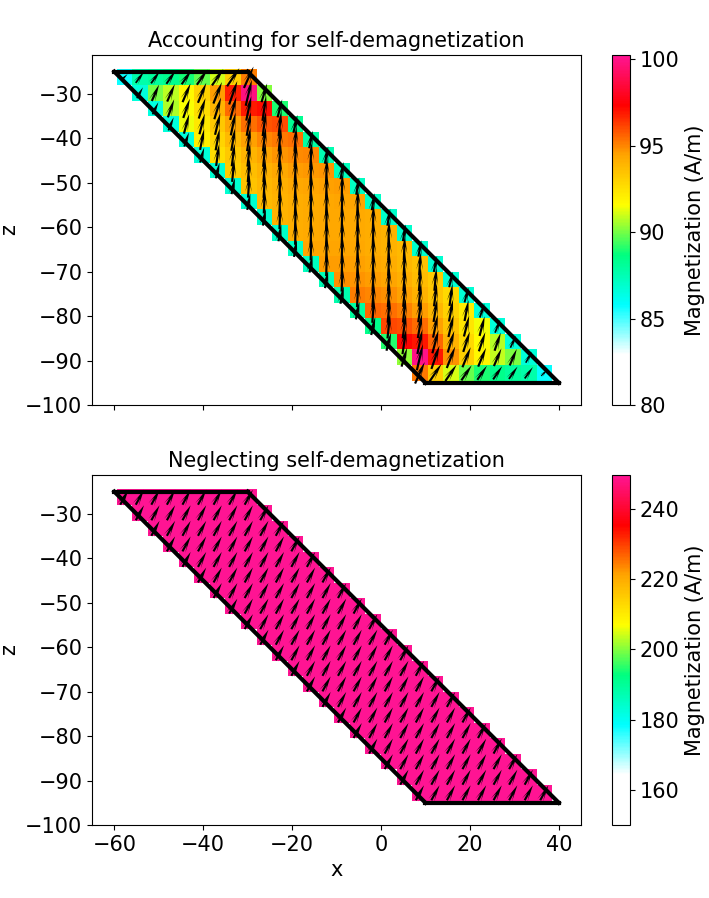
\includegraphics[width=\columnwidth]{figures/Magnetization.png}
    \end{center}
    \vspace{-0.5cm}
\caption{
    Computed magnetizations of a plate when accounting for self-demagnetization using the non-linear code (top panel) and when neglecting self demagnetization using the standard linear susceptibility code (bottom panel).
}
\label{fig:magnetization}
\vspace{-0.1cm}
\end{figure}



We first numerically compute the magnetization of the plate. Figure \ref{fig:magnetization} shows a cross section of the magnetization through the center of the plate computed from the nonlinear and linear forward modelings. When accounting for demagnetization with the nonlinear modeling (top panel), the magnetization is rotated away from the background geomagnetic field toward the long axis of the body. The amplitude of the magnetization is also significantly decreased throughout the plate. Although the magnetization is relatively uniform in amplitude and direction, variation in both can be seen near the edges of the plate. This is consistent with the fact that the demagnetizing field is in general non-uniform for non-ellipsoidal bodies \citep{Clark2014}.

Figure \ref{fig:TMI} shows a profile of TMI data running near the center of the plate. The data are simulated using both the linear forward modeling and nonlinear forward modeling. Additionally, data is simulated with magnetic vector forward modeling using the magnetization computed from the nonlinear forward modeling.  Figure \ref{fig:TMI}(a) shows a drastic reduction in the amplitude of the anomaly when applying the nonlinear forward modeling. This illustrates a saturation effect, whereby further increasing $\chi$ has a diminishing effect on $\mathbf{M}$. This indicates that the linear inversion code will grossly underestimate the susceptibility of highly susceptible targets. Figure \ref{fig:TMI}(b) shows the TMI data normalized by their respective maximums. The demagnetization significantly changes the characteristic of the TMI anomaly, indicating that the linear inversion will not only underestimate the susceptibility but will also alter the location of the plate in the recovered model. The alignment of the magnetic vector forward modeling with the nonlinear forward modeling in both panels illustrates the ability of MVI to model the demagnetization effect. To test the inversion algorithms, we simulate a grid of magnetic data 25 meters above the top of the plate, adding a small amount of random noise.
\begin{figure}[htb]
    \vspace{-0.1cm}
    \begin{center}
    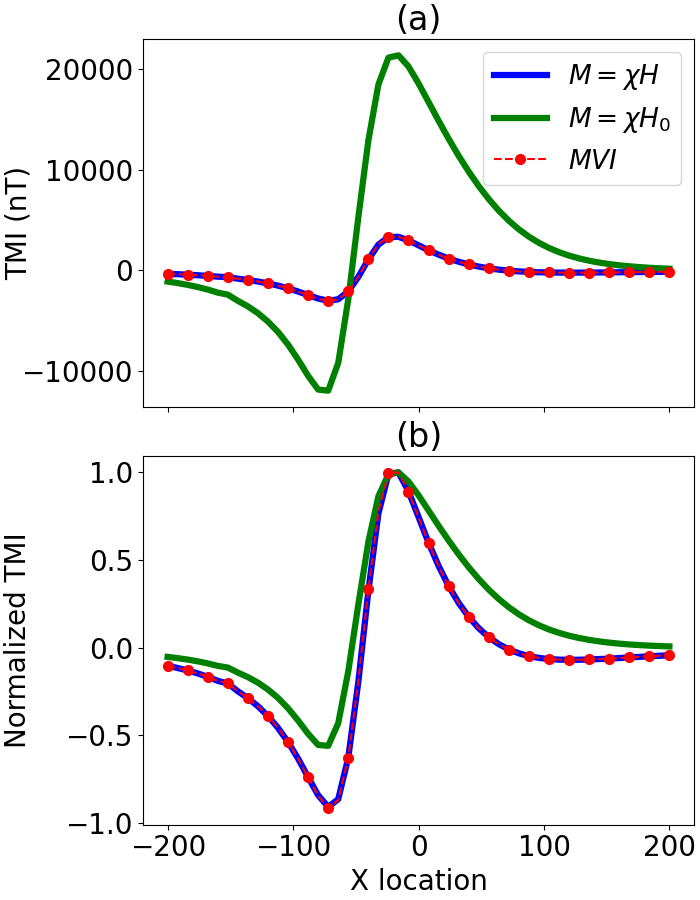
\includegraphics[width=\columnwidth]{figures/TMI.png}
    \end{center}
    \vspace{-0.5cm}
\caption{
    (a) Simulated TMI data running above the plate. The blue line is data accounting for demagnetization. The green line is data neglecting demagnetization. The red line is magnetic vector forward modeled data using the magnetization from the demagnetization corrected numerical solution.
    (b) The same data normalized by their respective maximum values.
}
\label{fig:TMI}
\vspace{-0.1cm}
\end{figure}

%\vspace{-0.45cm}
\section{Smooth Inversion}
%\vspace{-0.25cm}

 We formulate the inverse problem as an optimization problem with the objective function:\vspace{-0.1cm}
\begin{equation}
    \phi = \phi_d + \beta \phi_m
    \label{eq:phidphim}
    \vspace{-0.05cm}
\end{equation}
where $\phi_d$ measures how well the forward modeled data fits the true noisy data and $\phi_m$ is a regularization term  \citep{Oldenburg2005,Tikhonov1977}. $\phi_m$ has a general form of:\vspace{-0.1cm}
\begin{equation}
\phi_{\rm m} =
    {\alpha_s}\int w_s
    |m-m_{ref}|^p dv
     +
    \sum_{j=x,y,z}{\alpha_j}\int w_j
    \left|\frac{\partial m}{\partial i}\right|^q dv
\label{eq:model_regularization}
\end{equation}


where the first term punishes deviation from a reference model, and the remaining terms punish roughness in the model.

Potential field data has no inherent depth resolution, and the weighting functions $w_s$ and $w_j$  are set to counteract the decay of the fields and allow for models to be recovered at depth. While the depth weighting strategy of \cite{Li1996} is appropriate for the low susceptibility approximation, here we use sensitivity weighting to account for the nonlinear relationship between susceptibility and magnetization. This allows for the recovery of higher susceptibility values and compensates for the saturation effect discussed in the previous section.

The choice of $2$ for $p$ and $q$ in equation \ref{eq:model_regularization} is the commonly applied $\mathcal{L}_2$ norm for both the smallness and smoothness terms in the regularization. This choice of norm is computationally convenient but tends to punish outliers. This means inversion routines utilizing this choice of norm are often not able to recover models that are compact or that have sharp boundaries. Additionally, the $\mathcal{L}_2$ norm tends to underestimate the recovered physical property values \citep{Oldenburg2005,Sun2020}.

\begin{figure}[htb]
    \vspace{-0.1cm}
    \begin{center}
    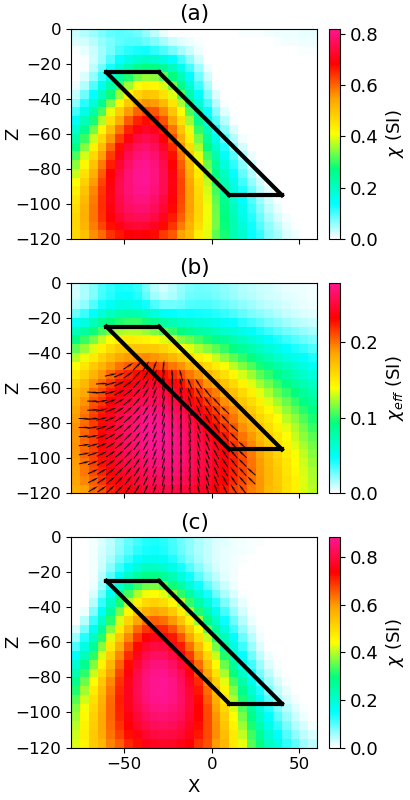
\includegraphics[width=\columnwidth]{figures/L2.png}
    \end{center}
    \vspace{-0.5cm}
\caption{
    Cross section through the recovered $\mathcal{L}_2$ models for each inversion method: (a) Linear, (b) MVI, (c) Nonlinear
}
\label{fig:L2}
\vspace{-0.1cm}
\end{figure}


We utilize the $\mathcal{L}_2$ regularization and invert the simulated geophysical data using a linear susceptibility inversion, MVI, and a non-linear susceptibility inversion. The recovered models are shown in Figure \ref{fig:L2}. Although all three recovered models place magnetic material in the right general location, they give poor indication of the dip and structure of the plate.  The linear inversion (Figure \ref{fig:L2}(a))  recovers a more vertical structure in the center of the plate. This is consistent with initial magnetic interpretations at Osborne, where not accounting for demagnetization indicated a more vertical dip and therefore misled drilling \citep{Clark2000}. The magnetic vector inversion (Figure \ref{fig:L2}(b)) is able to fit the data with a much smoother model with lower susceptibility values. This illustrates the additional ambiguity introduced in MVI due to the unconstrained magnetization direction. The nonlinear inversion (Figure \ref{fig:L2}(c)) only slightly improves the magnitude and location of the recovered susceptibility model as compared to the linear inversion.  At the recovered susceptibility values, the demagnetization effect is not significant, motivating the need to recover a more compact model.

%\vspace{-0.45cm}
\section{Sparse Norm Inversion}
%\vspace{-0.25cm}

The smooth inversion  results indicate that for compact bodies standard  $\mathcal{L}_2$ inversions may not adequately simulate demagnetization effects. To better recover a compact and sharper model we apply sparse norms to both the smallness and smoothness terms in equation \ref{eq:model_regularization}. To apply these norms we use the iteratively re-weighted least squares approach of \cite{Fournier2019}. This approach can approximate any value chosen for $p$ or $q$ between $0$ and $2$. For all three models we choose values of $1/2$ for $p$ and $q$. This choice of norm was empirically found to achieve the desired compactness and sharpness while not having the same tendency as the $L_0$ norm to become stuck in local minima. To apply sparsity to the Cartesian magnetic vector models, we implement the method of \cite{Ghalenhnoee2021} which enforces sparsity on the amplitude of magnetization rather than Cartesian components in the smallness term as follows:
\vspace{-0.1cm}
\begin{equation}
    \phi_{small} = \alpha_s \int w_s\left|\sqrt{m_x^2+m_y^2+m_z^2}\right|^p dv
\end{equation}

% \begin{equation}
%     \phi_{small} = \alpha_s \int w_s\left|{m}\right|^p dv
% \end{equation}
To enable the recovery of a more uniformly magnetized MVI model, we improve upon the smoothness term in this method by applying sparsity on the amplitude of the model gradients rather than on the gradient of the amplitude or the gradients of the individual Cartesian components:
% \begin{equation}
%     \phi_{smooth}=\sum_{j=xyz}{\alpha_j}\int w_j
%     \left|\sqrt{\sum_{k=xyz}\frac{\partial m_k}{\partial i}^2}\right|^q dv
% \end{equation}

\begin{equation}
    \phi_{small}=\frac{1}{2}{\alpha_s}\int
    |w_s m|^{p_s} dv
\end{equation}



Although the use of sparse norms can improve recovered models, they also can tend to over-compact recovered models \citep{Li2018}. This can be exacerbated by sensitivity weighting for the non-linear magnetic problem, as higher levels of susceptibility have a decreasing effect on the data, meaning that the corresponding sensitivity weights for highly susceptible cells will be lower. We therefore apply bound constraints to limit the upper value of susceptibility for the non-linear inversion.

\begin{figure}[htb]
    \vspace{-0.1cm}
    \begin{center}
    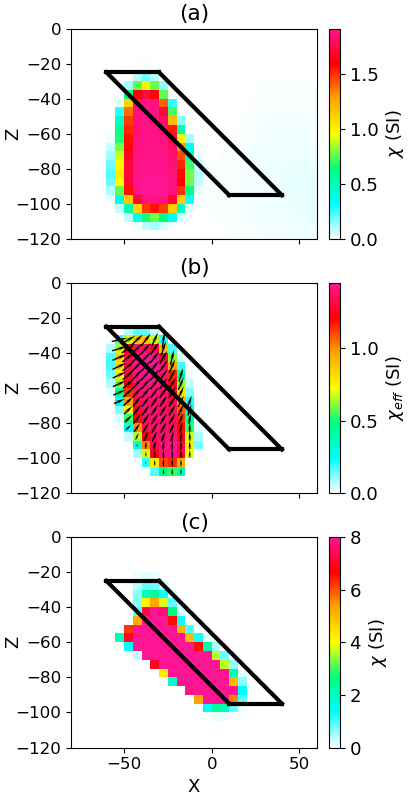
\includegraphics[width=\columnwidth]{figures/Lp5.png}
    \end{center}
    \vspace{-0.5cm}
\caption{
    Cross section of the recovered $\mathcal{L}_{1/2}$ models for each inversion method: (a) Linear, (b) MVI, (c) Nonlinear
}
\label{fig:Lp5}
\vspace{-0.1cm}
\end{figure}


Figure \ref{fig:Lp5} shows the sparse inversion results for the three different methods, where an upper bound of 8 SI has been applied to the non-linear susceptibility inversion. The low susceptibility inversion (Figure \ref{fig:Lp5}(a))  is now more compact and reaches slightly higher susceptibility values, but the general location and structure is consistent with the smooth linear model. This is because the direction of magnetization and resulting shape of the TMI anomaly is not altered by increasing the susceptibility values for the low susceptibility approximation. The sparse MVI model (Figure \ref{fig:Lp5}(b)) recovers a direction of magnetization that is mostly in line with the inducing field at the center of the target. As a result, it indicates a dip consistent with the linear approximation. The sparse nonlinear inversion (Figure \ref{fig:Lp5}(c))  is able to adequately replicate the self-demagnetization phenomenon of the plate at the high recovered susceptibility values. As a result, the nonlinear susceptibility model gives the best indication of the dip and structure of the plate. To test the sensitivity of the recovered model to bound constraints, we apply the nonlinear inversion approach with upper values of susceptibility of 2, 5, and 8 SI. While all three models do give a better indication of the dip, there is significant improvement in both the dip and volume of the recovered models for the susceptibility values within a few SI of the true susceptibility of the plate (6 SI).

\begin{figure}[htb]
    \vspace{-0.1cm}
    \begin{center}
    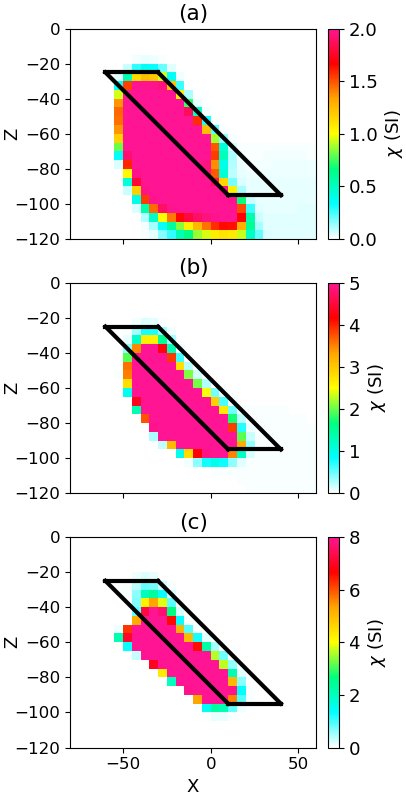
\includegraphics[width=\columnwidth]{figures/LpBound.png}
    \end{center}
    \vspace{-0.5cm}
\caption{
    Cross section of the recovered nonlinear $\mathcal{L}_{1/2}$ models using upper bound constraints of: (a) 2SI, (b) 5SI, (c) 8SI
}
\label{fig:Lp5bound}
\vspace{-0.1cm}
\end{figure}



%\vspace{-0.45cm}
\section{Discussion and conclusions}
%\vspace{-0.25cm}

While magnetic vector modeling and nonlinear forward modeling can account for demagnetization, there are inherent difficulties in each inversion method. Although the nonlinear inversion outperformed compact MVI in this circumstance, a significant amount of prior information was necessary to obtain the best inversion result.  We assumed that the susceptibility model was both compact and relatively uniform. Additionally, we assumed that our range of upper bounds for susceptibility was near to the true anomaly and that remanence and anisotropy were negligible.

If very high amplitude TMI anomalies or other geologic knowledge indicate that self-demagnetization effects could be present, running nonlinear susceptibility inversion with a variety of choices of norms and bound constraints can be a good way to test hypotheses. Additionally, the ability to run nonlinear susceptibility inversion in combination with MVI results can be a useful interpretive tool. If drill information is available, it can be used to constrain the high susceptibility inversion. It is not straightforward to include this information in MVI, as magnetization is influenced by the geometry of the body when susceptibilities are large.

\onecolumn


\bibliographystyle{seg}  % style file is seg.bst
\bibliography{self_demag}

\end{document}
